\chapter{Discussion}
\label{Discussion}
This section presents an analysis and discussion of the results. 

\section{Graph Behavior}
The behaviors shown represent typical trends observed when varying each parameter in the specified direction, but they may not apply to all possible values or reflect the magnitude of changes. 
Additionally, these results do not necessarily generalize to scenarios where two parameters are simultaneously varied. 
The graph behavior should be interpreted alongside the local $S1$ sensitivities from \Cref{sec:Sobol_sensitivity_analysis_results} to better understand how sensitive the output is to specific parameters and the potential impact of their variation.

A researcher would look at the growth curve and create their conclusions by visually looking at the curves and reasoning through the ODE model to explain the behavior. 
They can further supplement this analysis with a Sobol analysis to quantify how significant the change was, and compare a parameter's significance with other parameters. 

\section{Realistic Growth Curves}
As the complexity of the network grows, biologically accurate curves might disappear. 
In a $1\times 1\times 1$ system, like that in \Cref{fig:created:a_good_curve}, there is a clear exponential growth, peak, and death cycle for the bacteria. 
The phages experience a delay in growth, but also exhibit exponential growth. 
These behaviors can disappear as the community size grows to a $p\times b\times r$ system. 
\Cref{fig:created:large_graph_network_output} shows how these behaviors disappear. 
Some, but not every phage or bacteria in \Cref{fig:created:large_graph_network_output} exhibits a clear growth and death cycle. 
Bacteria face increased competition for resources, and phages face increased competition for bacteria. 
This increased competition decreases the pool of available resources for the bacteria and phages to grow. 
There is an external threat, the washout, so any bacterial and phage growth gets cancelled out by the washout, or even worse, if the growth is not fast enough, completely eliminated. 

There are only 2 interactions that occur in a $1\times1\times1$ system. 
With a $p\times b\times r$ system, there are at most $p\cdot b + b\cdot r$ interactions that can occur. 
Any number of phages can interact with any number of bacteria, and any number of bacteria can interact with any number of resources, each with their own unique parameter values. 
These varying rates will influence the dynamics of the system, and make it hard to determine what event caused what due to the rise in number of interactions.
With so many individual events occurring at the same time, it makes harder to identify the cause of the event, and how the event's action will propagate through the network. 

There are ways to circumvent this issue. 
Simulations offer the ability for researchers to experiment with the system that normally might not be feasible. 
Knocking out certain nodes or edges and rerunning the simulation would allow the researcher to see how the knocked out node or edge influenced the simulation. 
The knocked out node or edge won't contribute to the simulation anymore, so there will be an impact on the population count. 
The larger the difference, the more important that that node or edge had on the simulation. 

\subsection{Knockout}
\Cref{fig:created:large_graph_network_output_hidden_B14_P2} and \Cref{fig:created:large_graph_network_output_knockout_B14_P2}
show the difference that a knockout has on the output of the graphs. 
$P_2$ and $B_14$ were knocked out of the network, using \Cref{fig:ss:example_large_network} as the base network. 
On average, there are more resources, as there is less competition for the resources. 
In the knocked out graph, more bacteria were able to survive, and in total there were more bacteria in the system as evident by the bacteria sum. 
There are also less infected bacteria. 
With the phages, there is less of an obvious difference in behavior, but in \Cref{fig:created:large_graph_network_output_hidden_B14_P2}, $P_18$, pink, suddenly increases in population at $t=10$ until the end of the simulation, while this doesn't happen in \Cref{fig:created:large_graph_network_output_hidden_B14_P2}. 
$P_18$ infects $B_14$ (as well as $B_13$), so by removing $B_14$ $P_18$ was negatively affected. 

By removing $P_2$ and $B_14$, it was casually shown how the resource, bacteria, and phage dynamics were permanently altered. 
\Cref{fig:created:large_graph_network_output_knockout_B14_P2} showed how knockouts have a lasting impact on the dynamics of the system, changing which phages and bacteria survive. 
\begin{figure}
    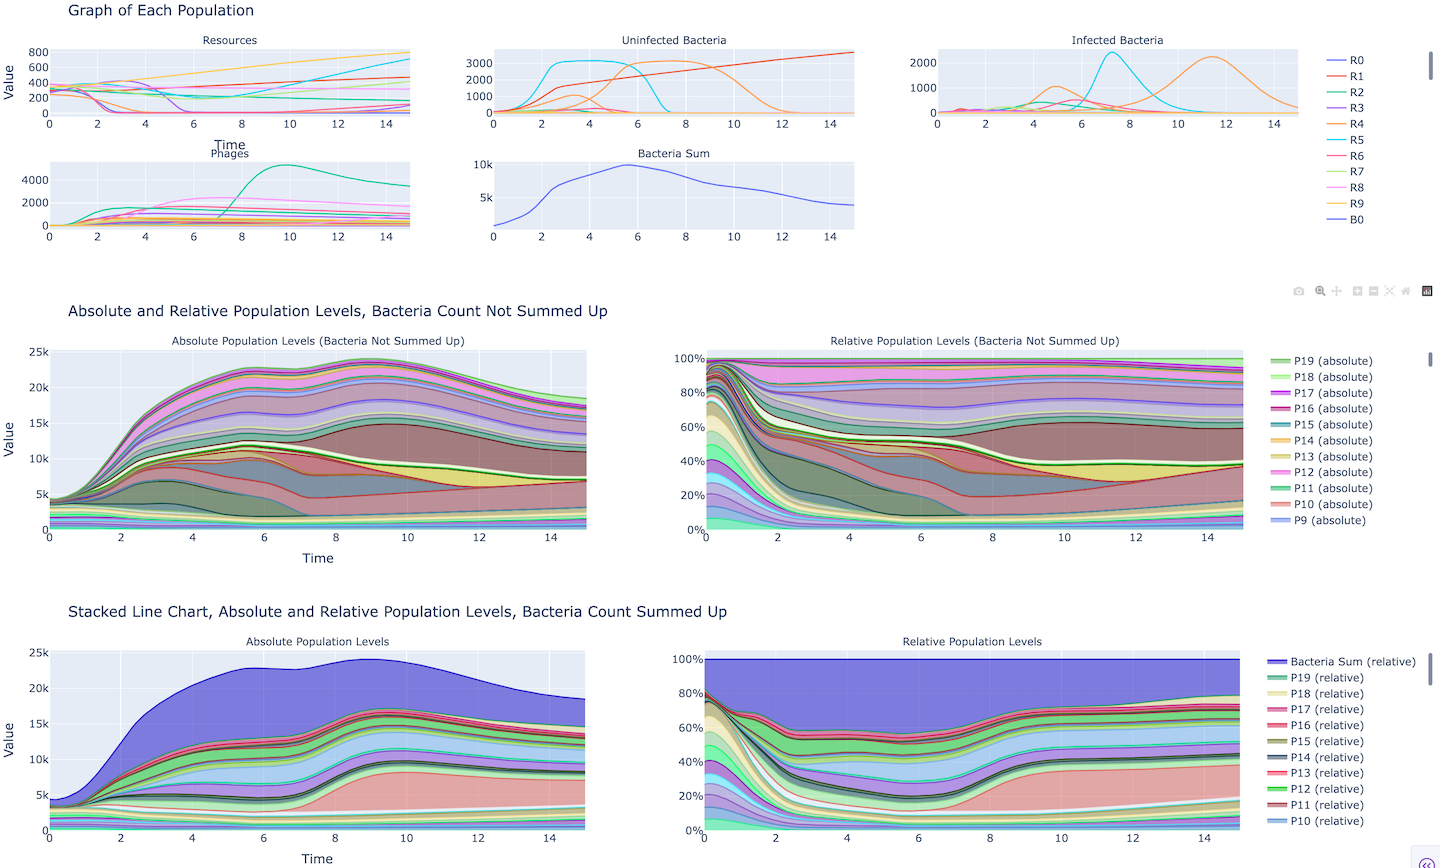
\includegraphics[width=1\textwidth]{Plots/Created/large_graph_network_output.png}
    \centering
    \caption{
        The output graph for the default parameter values for a large $20\times 20 \times 10$ network. 
        Parameter values were randomly chosen in the interval given by \Cref{tab:appendixE:Sobol_analysis_values}. 
    }
    \label{fig:created:large_graph_network_output}
\end{figure}

\begin{figure}
    \centering
    \begin{subfigure}{0.49\linewidth}
        \centering
        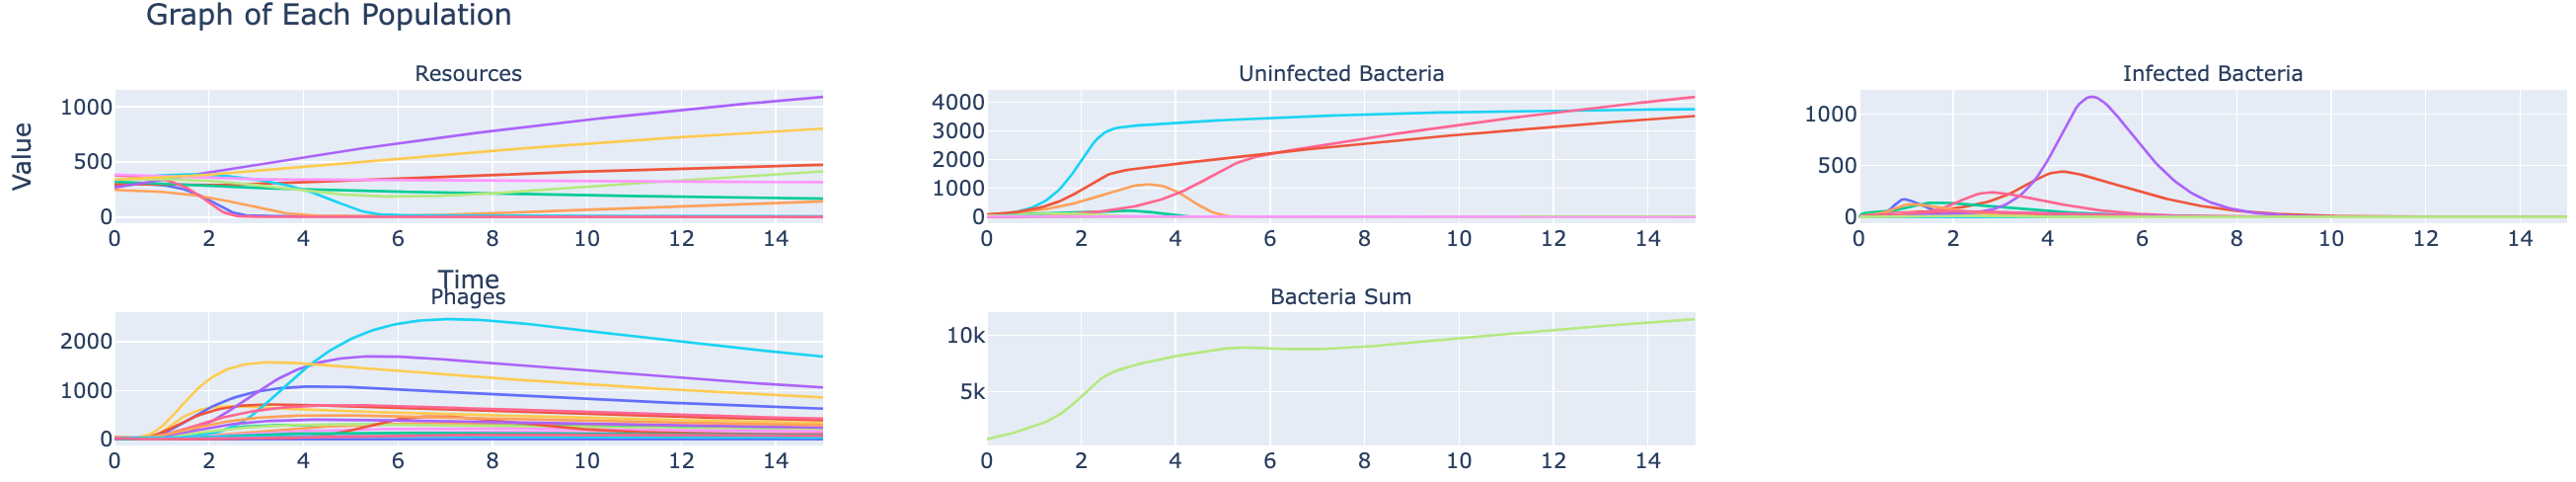
\includegraphics[width=\linewidth]{Plots/Created/large_graph_network_output_knockout_B14_P2.png}
        \caption{
            The same figure as \Cref{fig:created:large_graph_network_output}, but with phage $P_2$ and bacteria $B_14$ hidden from the graph. 
        }
        \label{fig:created:large_graph_network_output_hidden_B14_P2}
    \end{subfigure}
    \hfill
    \begin{subfigure}{0.49\linewidth}
        \centering
        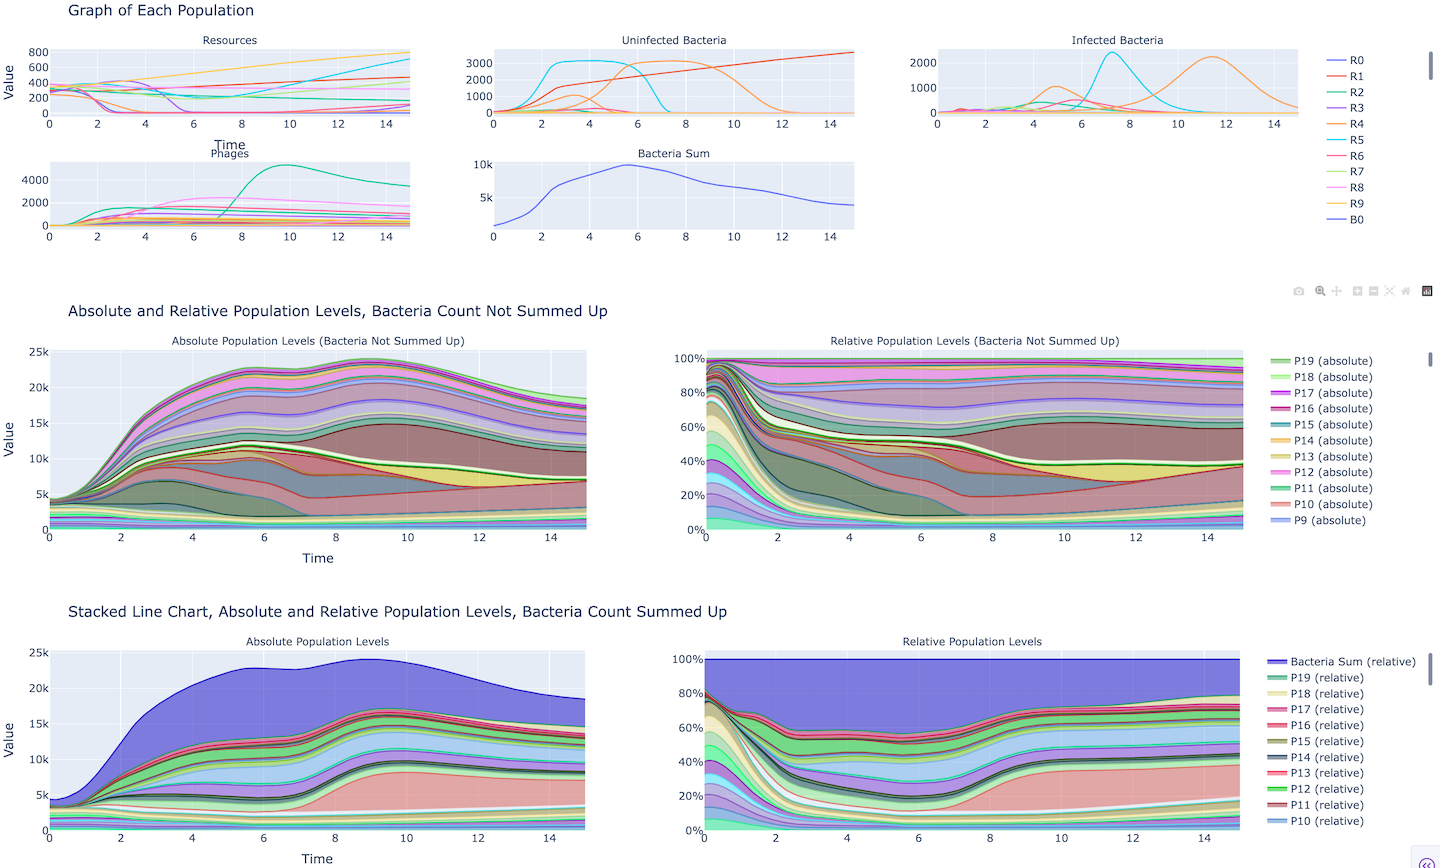
\includegraphics[width=\linewidth]{Plots/Created/large_graph_network_output.png}
        \caption{
            The large $20\times 20\times 10$ network, with phage $P_2$ and bacteria $B_14$ knocked out from the system.
        }
        \label{fig:created:large_graph_network_output_knockout_B14_P2}
    \end{subfigure}
    \caption{
        Comparing the effect of knocking $P_2$ and $B_14$ out from the system. 
        Figure a) has $P_2$ and $B_14$ hidden from the system, while Figure b) has the phage and bacteria knocked out from the system. 
        The most important phage and bacteria as noted by the bacteria growth were knocked out. 
        \Cref{fig:ss:example_large_network} is used as the reference network model. 
        The colors between a) and b) can not be directly compared as the color is not mapped to a specific phage or bacteria. 
    }
\end{figure}

\section{Sobol Sensitivity}
A researcher might have an intuitive understanding of how a model works, but might be unsure of how important the parameters of the model has on the model results.  
A researcher can use Sobol to quantify how important a change in parameter value is in the context of the simulation results. 
By testing and measuring hundreds of simulation inputs and outputs, Sobol understands how changing a parameter value would influence the output of the parameter. 
By identifying the important parameters, a researcher could use that to their benefit in their research. 
Researchers can prioritize adjusting the most influential parameters in their simulations or consider engineering phages and bacteria to achieve the desired parameter values.

\subsection{Resources}
Every parameter affects how the bacteria and phage population grows in some way, which influences the consumption rate of resources, which determines the final resource value. 
Of the other parameters, $\tau$ has the biggest influence because $\tau$ determines how fast the bacteria will go through the infection process. 
The longer it takes, the longer it takes for the phage population to grow, allowing more bacteria to grow and consume resources. 

\subsection{Phages}
The $r$ value quantifies how fast the phages infect the uninfected bacteria. 
$r$, the adsorption rate of phages to bacteria, can be interpreted as the efficiency of infection. 
The smaller the value, the more efficient the infection process is, and fewer phages it requires to infect a bacterium. 
With a larger $r$ value, more phages are used to infect a bacterium. 
$\beta$ has an influence on the final phage population, as the infected bacterium will release $\beta$ phages into the system. 
The more phages that are created for every lysed bacterium, the more phages are available in the system. 

The barplot values for the peak value for phages using the 95\% rule has the same values as in the final value plot for the phages. 
This makes sense as there is no removal of phages from the system, so any phages created by $r$ or $\beta$ will stay in the system. 
As the population is ever-increasing, the final and peak value will be occurring near one another and are tightly associated with one another.

The $\tau$ parameter influences how fast an infected bacterium goes through the infection process. 
Decreasing tau increases the speed of lysis, allowing more phages to be produced faster. 
This in turn will increase the phage population faster than other parameters, meaning that the phages reached the peak population faster.
$r$ and $\beta$ have similar effects, but rather have a larger effect on the final and peak phage population than the time it takes to reach the peak value. 
$r$ and $\beta$ add to the phage population, rather than specifically speed up a process which $\tau$ does. 
Decreasing $r$ and increasing $\beta$ lead to more phages being created, which can then infect more bacteria. 
This won't have nearly as large of an impact as shortening the infection period, literally decreasing the time until new phages are created, thus causing the phage population to reach its peak faster. 

\subsection{Total Bacteria}
Resources, $\tau$, $e$, and $\beta$ all play a critical role in the final population value of bacteria. 
More resources allow bacteria to grow for a longer time, allowing more bacteria to be created. 
$\beta$ has a very important role in determining the final bacteria population, but surprisingly $r$ has no role in determining the final bacteria population. 
$e$ determines the resource consumption rate. 
The larger $e$ is, the faster the depletion rate of the resource. 
So by lowering $e$, more bacteria will be created, and the time at which the bacteria peak at occurs later in time. 
Of course as $\beta$ changes value, it will have a large influence on the final bacteria population. 
More phages will cause more infections, slowing the spread of bacteria. 
However, $r$ surprisingly does not have an influence on the final bacteria population level.  

The total bacteria peak population is much more sensitive to the different parameter values. 
The bacteria act as a link between the phages and resources. 
Any changes in the resource consumption rate or initial condition will affect the bacteria population. 
Likewise, any change in phage adsorption rate will affect the bacteria growth, which in turn will affect the resource consumption rate. 
The bacteria have the ability to dampen the effect of certain parameters. 
For example, the initial resource value affects the final resource value. 
The initial resource value partially affects the final bacteria value, but it doesn't affect the phages. 
The parameters lose strength as it propagates through the system. 

Since the bacteria exist in the middle between the phages and resources, the bacteria are exposed to many different parameters that will ultimately influence the peak value. 
Many of these parameters are interacting with one another hence why $ST > S1$ is true for many of the inputs. 

Similar to the peak value, the bacteria interact with many parameters, who interact with other parameters. 
The time of the peak can only occur between $t=0$ and the end of the simulation, limiting the values that can be measured, reducing the potential variance seen in the output. 
The peak value on the other hand has no limit on the peak value, with a peak value occurring anywhere between 0 and $\infty$. 
$e$ and $K$ depend almost exclusively on higher order terms due to the nature of the bacteria growing at the Monod rate. 

\section{Initial Value Analysis}
The behavior between \Cref{fig:created:initial_value_analysis_UB_50_500_a_good_plot_2} and \Cref{fig:created:initial_value_analysis_UB_50_500_a_good_plot} should be similar, however the change in parameter values altered the simulation to introduce a region in behavior change. 
It would be expected that for 100 initial uninfected bacteria and less the bacteria sum peak time would follow the linear regression line, but at around 100 uninfected bacteria and less, the peak curve deviated from the linear expression. 

Between 100 and 500 uninfected bacteria, the system is adsorption limited. 
The adsorption of phages to bacteria depends on the bacterial concentration \cite{mullaExtremeDiversityPhage2024}. 
There are not enough phages relative to the population to infect the bacteria, so the phages slowly adsorb to the bacteria. 
The bacteria can grow without immediate pressure from the phages. 
There is also a lack of resources which is restricting the bacterial growth. 
For large initial bacteria concentrations, the resources run out. 
This severely limits the ability for the bacteria to grow and artificially limits the population cap of the bacteria. 

The system is latency limited between 25 and 100 uninfected bacteria. 
The collapse time in a latency limited regime is independent of the initial bacteria population \cite{mullaExtremeDiversityPhage2024}.
As the initial bacteria decreases, $r\cdot \beta$ eventually becomes smaller than $1/tau = \frac{1}{2.14} = 0.467$, that's around where the transition happens - see Yuval's paper supplement.the phage to bacteria ratio increases, and they can infect the bacteria faster. 
So the time to phage peak also decreases as the initial uninfected bacteria decreases. 

As the uninfected bacteria decreases from 25 towards 1, it takes longer for the bacteria to grow and reach their peak population count. 
At these initial bacteria concentration levels, there is enough resources to fully sustain the bacteria through the whole simulation. 
For uninfected bacteria less than 25, the system enters a new sort of restriction, where the system experiences a delayed in infection due to low encounter rates. 

The transition rate from $U$ to $I_1$ is proportional to $U\cdot P$. 
Fewer bacteria are initially infected with a low initial starting bacteria. 
If the phages can't infect the bacteria, the later infection stages are delayed due to the slow infection process. 
There could be a threshold for phage to uninfected bacteria where a certain dilution rate will significantly affect the peak time. 
This value could be around $\frac{\text{initial phage}}{\text{initial bacteria}} = \frac{10}{25} = 0.4$ as at around 25 uninfected bacteria is when the system switches from latency limited to the new limited regime. 
The bacteria have a longer amount of time to grow as there is a low infection rate and plenty of resources to consume. 
This means that it takes longer for the bacteria to grow, as noticed by the increase in peak time relative to larger initial uninfected bacteria populations. 
As the bacteria population drives the phage population, an increase in bacteria time of peak causes an increase in phage time of peak. 

\section{Phage Proliferation}
\subsection{Phase Portrait}
There is non-linear trade-off between initial resources and initial phages when there is washout included. 
The washout non-linearly affects if the phages proliferate or not. 
The bigger the washout value, the harder it is for the phages and bacteria to proliferate. 
The bacteria couple the phage populations to resources, so changes in initial resource concentration will have an effect on the final phage value. 
Increasing the initial resource concentration creates more bacteria, while decreasing it results in fewer bacteria.
More bacteria ultimately produce more phages, while fewer bacteria ultimately result in fewer phages.
While Sobol with washin and washout, \Cref{fig:created:Sobol_peak}, showed that the final value for phages due to changes in initial resource input values is limited (sensitivity $\approx 0.1$), it still has an impact. 

For low initial resource concentration values, values below $10$ the resource, the Monod curve is below the half-velocity constant (the velocity $v$ is 1 and $K$ is 10). 
The lack of resources restricts the bacteria growth, and the bacteria can't grow quickly. 
As the resource concentration increases towards $K=10$, the bacteria can grow faster. 
Since $K$ is small, a small change in $R$ causes a relatively large change in the Monod rate. 

At around the minimum in the phage proliferation boundary, the behavior changes. 
The minimum happens at $R\approx 7$, the Monod rate reaches half of its max velocity. 
This behavior should be seen at around 10, but the washout has an effect on the Monod rate by artificially shifting the point where the half velocity occurs from $K=10$ to $K\approx 7$. 
$10\cdot 0.98^{15} = 7.386$

As $R$ increases from $K$, the bacteria are not limited by the nutrients anymore and can grow faster. 
However, as $R$ increases beyond $K$, each additional unit of $R$ results in a diminishing increase in the Monod rate, which asymptotically approaches its maximum velocity. 
As bacteria grow according to the Monod equation $g(N, v, K)$, the phage population dynamics remain tightly coupled to bacterial growth. 

Phage proliferation becomes a race against time under external pressure. 
The phages will not proliferate if the phage growth rate is not fast enough to initially beat the washout removal rate, or the infected bacteria are washed out before lysing. 

\subsection{3D Plot}
It is difficult to see inside the matrix, but using the color on the outside can give some insights into the behavior happening inside the matrix. 
Even with the added bacteria, the phage proliferation boundary is still heavily dependent on the initial phages and initial resources, and less so on bacteria. 

\section{Plotting Parameter Change}

\section{Phage and Bacteria Survivability}
There are so many interactions and parameters in large and complex systems that it becomes hard to analyze. 
The model network and parameter values are relatively random, and a figure of the network interactions and a copy of the parameter inputs is needed in order to have some sort of chance to analyze why a phage or bacteria is behaving in a certain way. 
Further, it is hard to simplify the model, for example by knocking out unimportant bacteria from the system, due to the interconnected nature of the system. 


Since their discovery, bacteriophages have been traditionally regarded as the natural enemies of bacteria. However, recent advances in molecular biology techniques, especially data from "omics" analyses, have revealed that the interplay between bacterial viruses and their hosts is far more intricate than initially thought. On the one hand, we have become more aware of the impact of viral predation on the composition and genetic makeup of microbial communities thanks to genomic and metagenomic approaches. Moreover, data obtained from transcriptomic, proteomic, and metabolomic studies have shown that responses to phage predation are complex and diverse, varying greatly depending on the bacterial host, phage, and multiplicity of infection. Interestingly, phage exposure may alter different phenotypes, including virulence and biofilm formation. The complexity of the interactions between microbes and their viral predators is also evidenced by the link between quorum-sensing signaling pathways and bacteriophage resistance. Overall, new data increasingly suggests that both temperate and virulent phages have a positive effect on the evolution and adaptation of microbial populations. From this perspective, further research is still necessary to fully understand the interactions between phage and host under conditions that allow co-existence of both populations, reflecting more accurately the dynamics in natural microbial communities.

Phages have traditionally been seed as the enemy of bacteria, but with new trancriptomic, proteomic, genomic, and metabolomic methods, we have a better understanding of hoe phage predation infleunces 

Overall, new data increasingly suggests that both temperate and virulent phages have a positive effect on the evolution and adaptation of microbial populations. From this perspective, further research is still necessary to fully understand the interactions between phage and host under conditions that allow co-existence of both populations, reflecting more accurately the dynamics in natural microbial communities. 

\subsection{Ecology}
With the competitive exclusion principle in ecology, there should be at most 10 surviving bacteria. 
Two or more species competing for the same resources can not coexist indefinitely. 

The $\text{R}^{*}$ resource-ratio hypothesis rule is a rule that states that a species needs to be the best at consuming resources to persist. 
The growth rate of a species is proportional to the resources consumed with an energy factor, minus a maintenance and death rate. 
The bigger the resource overlap between competing bacteria, the smaller the realm of co-existence \cite{vandenbergEcologicalModellingApproaches2022}. 

\subsection{Debris Term}
\label{sec:discussion:debris}
A recently published paper \citet{deyEmergentHigherorderInteractions2025} uses the Golding model but adds a new term, debris. While running their simulations and experiments, the model's results would diverge from their experimental work. 
Their thinking is that freshly lysed bacteria still have biomarkers that phages can detect and attach to. 
Incorporating the debris term, which acts as an additional sink for phages, improved the model's alignment with the experimental data.
The debris term can also encompass bacterial phage defenses (\Cref{sec:literaturereview:bacterial_defense_against_phages}). 
The phage equation from the Golding model can be rewritten as 
\[
    \frac{dP_p}{dt} = \sum_{b\in B}\beta_{p b}\cdot\frac{M}{\tau_b} \cdot I_{b_M} - r_{p b}\cdot(U_b + \sum_{k=1}^{M} I_{b_k})\cdot P_p - w^o \cdot P_p \mathcolor{red}{- d_{p, b} \cdot P_p}
\]
\Cref{fig:created:debris_model} shows how debris $d$ had an effect on the growth curves of the phages and bacteria in comparison to no debris term, \Cref{fig:created:no_debris_model}. 
Without the debris term, only one uninfected bacteria survived, and every phage survived except for one phage who died due to the washout. 
Three uninfected bacteria species reached more than 1000 uninfected bacteria at any point in the simulation time, and only two infected bacteria species reached more than 1000 infected. 
The maximum total bacteria population that was reached was a total of 6620 bacteria. 

With the debris term included, different results are obvious. 
Three uninfected bacteria survived, four different uninfected bacteria strains ever reached a population value of greater than 1000 at any point in time during the simulation. 
Only one bacteria strain ever reached more than 1000 infected bacteria, 
The ending bacteria value is 12000, almost double the maximum bacteria population reached without debris. 
On average, there were significantly fewer phages at the end of the simulation than without debris. 
No phage population ended above 2000 with debris, while without debris two phage populations ended up with more than 2000 phages. 

\begin{figure}
    \centering
    \begin{subfigure}{1\linewidth}
        \centering
        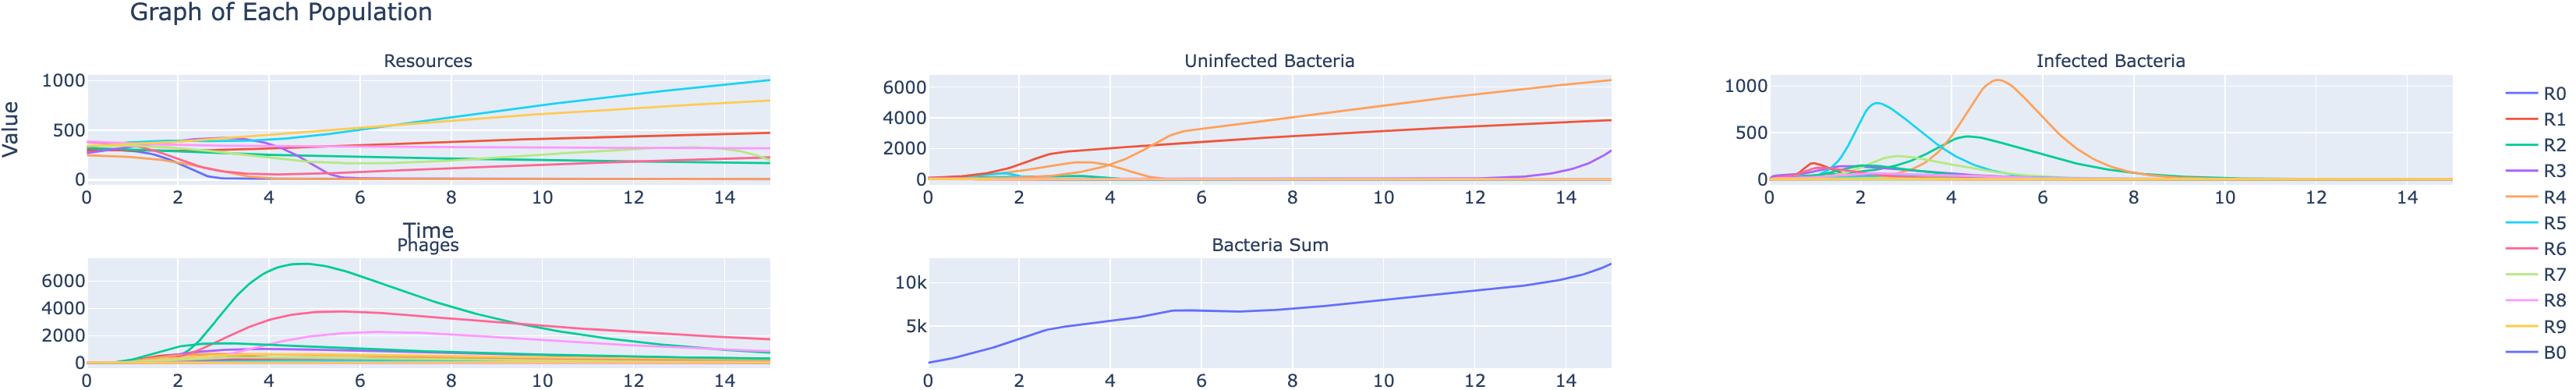
\includegraphics[width=\linewidth]{Plots/Created/debris.png}
        \caption{
            The $20\times20\times10$ model with a debris factor included. 
        }
        \label{fig:created:debris_model}
    \end{subfigure}
    \hfill
    \begin{subfigure}{1\linewidth}
        \centering
        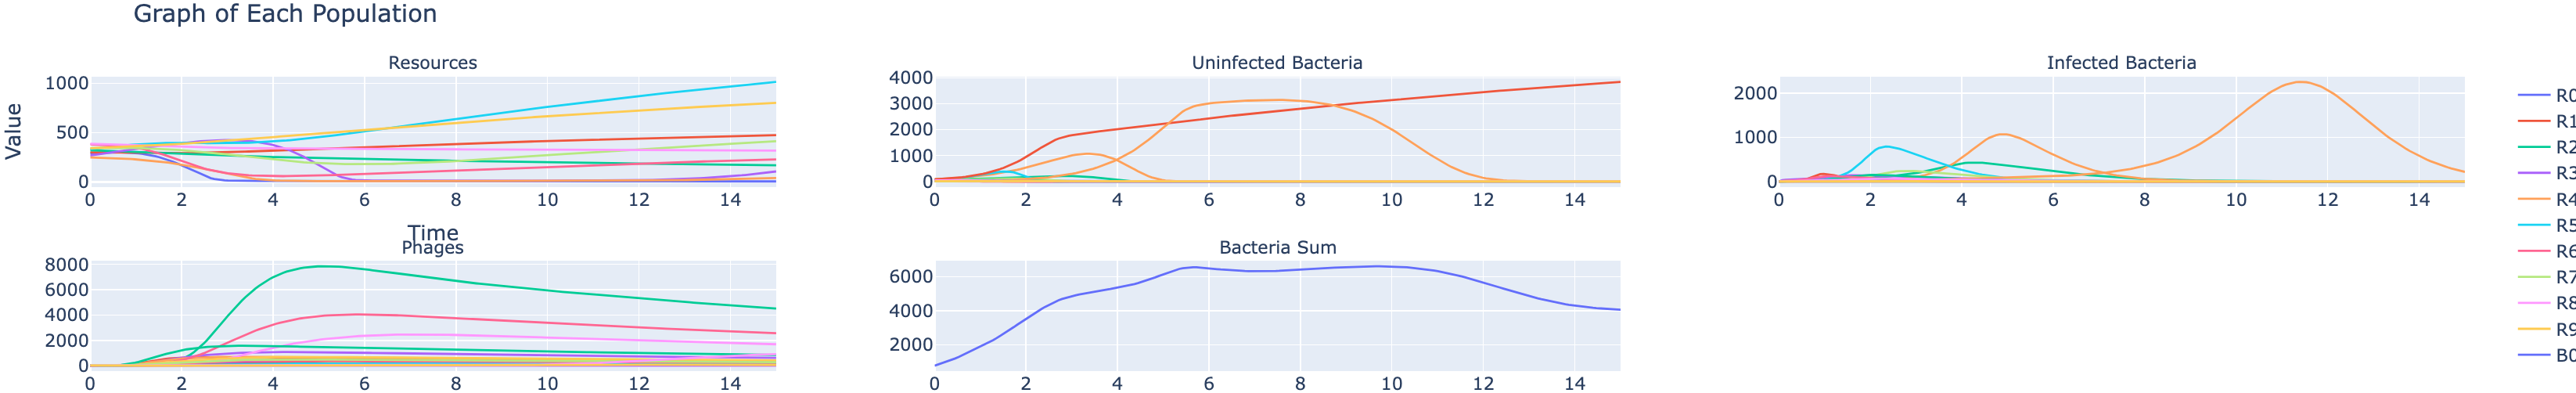
\includegraphics[width=\linewidth]{Plots/Created/no_debris.png}
        \caption{
            The $20\times20\times10$ model without the debris factor included. 
        }
        \label{fig:created:no_debris_model}
    \end{subfigure}
    \caption{
        A large $20\times20\times10$ model with a debris model added. 
        The debris parameter values were randomly and uniformly selected between 0.01 and 0.2.
    }
    \label{fig:created:debris}
\end{figure}